\setAuthor{Jaan Kalda}
\setRound{lõppvoor}
\setYear{2018}
\setNumber{G 9}
\setDifficulty{8}
\setTopic{Elektriahelad}

\prob{Kondensaator}
\begin{wrapfigure}[7]{r}{0.3\linewidth}
\vspace{-10pt}
\begin{center}
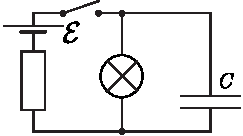
\includegraphics[width=\linewidth]{2018-v3g-09-LC-Q}
\par\end{center} 
\end{wrapfigure}

Vaatleme joonisel kujutatud elektriskeemi, mis koosneb kondensaatorist mahtuvusega $C$, patareist elektromotoorjõuga $\mathcal{E}$, takistist ja hõõglambist, mida võib lugeda mittelineaarseks takistiks (pinge sõltub voolust mittelineaarselt). Algselt oli kondensaator laenguta ja lüliti oli avatud. Seejärel suleti lüliti lühikeseks ajaks, misjärel see avati uuesti ning hoiti lahtisena seni, kuni kondensaator oli täielikult tühjenenud. Selle aja jooksul, mil lüliti oli suletud, eraldus kogu skeemil soojushulk $Q_1$; lüliti avamise järel eraldus täiendavalt veel soojushulk $Q_2$. Leidke laeng, mis läbis hõõglambi sel perioodil, kui lüliti oli suletud.

\hint
Pärast lüliti avamist eraldub kogu energia kondensaatorilt lambis soojusena. Lisaks on kogu vabanev soojusenergia võrdne patarei kogutööga.

\solu
Teises staadiumis eralduv soojus on võrdne kondensaatori energiaga lüliti avamise hetkel, $Q_2=q_C^2/2C$, kus $q_C$ on kondensaatori laeng sel hetkel. Kogu vabanev soojusenergia on võrdne patarei kogutööga
\[
A=(q_C+q_R)\mathcal E=Q_1+Q_2,
\]
kus $q_R$ on otsitav lampi läbiv laeng. Seega
\[
q_R=\frac{Q_1+Q_2}{\mathcal E}-\sqrt{2CQ_2}.
\]

\probeng{Capacitor}
\begin{wrapfigure}[7]{r}{0.3\linewidth}
\vspace{-10pt}
\begin{center}
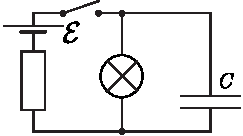
\includegraphics[width=\linewidth]{2018-v3g-09-LC-Q}
\par\end{center} 
\end{wrapfigure}
Let us look at the circuit diagram in the drawing, which is made of a capacitor of capacity $C$, a battery with an electromotive force $\mathcal{E}$, a resistor and an incandescent lamp which can be looked at as a non-linear resistor (the voltage’s dependence on the current is non-linear). At first the capacitor had no charge and the switch was opened. Next, the switch was closed for a short time, after that it was opened again and was held open until the capacitor was completely emptied. During the time when the switch was closed, a heat $Q_1$ was dissipated by the whole circuit; after opening the switch an additional heat $Q_2$ was dissipated. Find the charge that went through the incandescent lamp when the switch was closed.

\hinteng
After opening the switch all of the energy leaves the capacitor as heat from the lamp. In addition all the released thermal energy is equal to the total work of the battery.

\solueng
The heat dissipated in the second stadium is equal to the capacitor’s energy at the moment of opening the switch, $Q_2=q_C^2/2C$ where $q_C$ is the capacitor’s charge at this moment. The total thermal energy released is equal to the total work of the battery $A=(q_C+q_R)\mathcal E=Q_1+Q_2$ where $q_R$ is the desired charge going through the lamp. Therefore $q_R=\frac{Q_1+Q_2}{\mathcal E}-\sqrt{2CQ_2}$.
\probend